\section{Applying RISE}
\nblink{nhs-chest-xray/analyze/rise.ipynb}
\nblink{nhs-chest-xray/analyze/rise\_bounding\_boxes.ipynb}

The implementation of RISE on the NIH Chest X-ray dataset with the DenseNet model was straightforward, because the reference implementation of RISE on GitHub \cite{risegithub} already
contained a working implementation for PyTorch. The implementation was not published on the Python Packaging Index, so the code had to be downloaded and added into our GitHub repository.

\subsection{Results}
\begin{figure}[H]
\centering
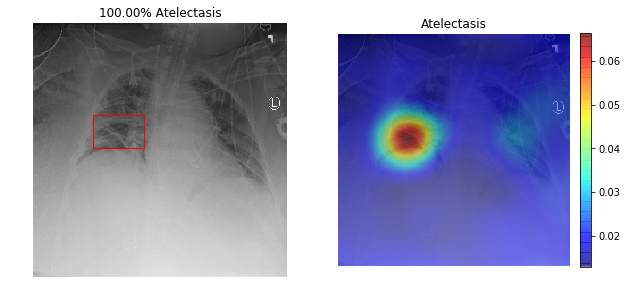
\includegraphics[width=12cm]{chapters/03_classification/images/rise_0.png}
\caption{The left image shows the input image with the bounding box added by a physician. The right image shows a RISE heat map and proofs that the neural network considers the correct part of the image as relevant for the correct classification}
\label{rise_example_1}
\end{figure}

\begin{figure}[H]
\centering
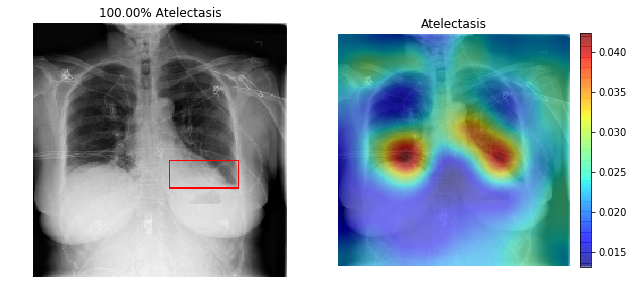
\includegraphics[width=12cm]{chapters/03_classification/images/rise_2.png}
\caption{The left image shows the input image with the bounding box added by a physician. The right image shows a RISE heat map and showing multiple regions that where important for the correct classification of this image.}
\label{rise_example_2}
\end{figure}

\begin{figure}[H]
\centering
\caption{RISE example 3}
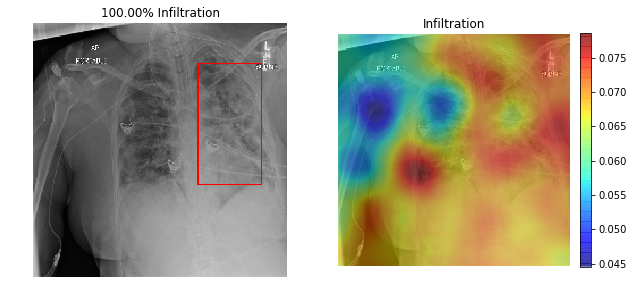
\includegraphics[width=12cm]{chapters/03_classification/images/rise_8.png}
\label{rise_example_3}
\end{figure}

\subsection{Discussion}
Figure \ref{rise_example_1} shows that the bounding box created by a physician perfectly matches the region the neural network looked to came to the correct classification. In comparision, in Figure \ref{ri


Looks good for most, some (like the last image) are very bad.
